% Customizable fields and text areas start with % >> below.
% Lines starting with the comment character (%) are normally removed before release outside the collaboration, but not those comments ending lines

% svn info. These are modified by svn at checkout time.
% The last version of these macros found before the maketitle will be the one on the front page,
% so only the main file is tracked.
% Do not edit by hand!
\RCS$Revision: 240525 $
\RCS$HeadURL: svn+ssh://svn.cern.ch/reps/tdr2/notes/DN-14-008/trunk/DN-14-008.tex $
\RCS$Id: DN-14-008.tex 240525 2014-05-06 12:16:46Z alverson $
%%%%%%%%%%%%% local definitions %%%%%%%%%%%%%%%%%%%%%
% This allows for switching between one column and two column (cms@external) layouts
% The widths should  be modified for your particular figures. You'll need additional copies if you have more than one standard figure size.
\newlength\cmsFigWidth
\ifthenelse{\boolean{cms@external}}{\setlength\cmsFigWidth{0.85\columnwidth}}{\setlength\cmsFigWidth{0.4\textwidth}}
\ifthenelse{\boolean{cms@external}}{\providecommand{\cmsLeft}{top}}{\providecommand{\cmsLeft}{left}}
\ifthenelse{\boolean{cms@external}}{\providecommand{\cmsRight}{bottom}}{\providecommand{\cmsRight}{right}}
%%%%%%%%%%%%%%%  Title page %%%%%%%%%%%%%%%%%%%%%%%%
\cmsNoteHeader{DN-14-008} % This is over-written in the CMS environment: useful as preprint no. for export versions
% >> Title: please make sure that the non-TeX equivalent is in PDFTitle below
\title{A new trigger concept for muons in the barrel region of the CMS experiment: Muon Track fast Tag}

% >> Authors
%Author is always "The CMS Collaboration" for PAS and papers, so author, etc, below will be ignored in those cases
%For multiple affiliations, create an address entry for the combination
%To mark authors as primary, use the \author* form
\address[neu]{RWTH Aachen University}
\author[neu]{Yusuf Erdogan}
\author[neu]{G\"unter Fl\"ugge}
\author[neu]{Thomas Hebbeker}
\author[neu]{Andreas K\"unsken}
\author[neu]{Erik Dietz-Laursson}
\author[neu]{Markus Merschmeyer}
\author[neu]{Oliver Pooth}
\author[neu]{Thomas Rademacher}
\author[neu]{Florian Scheuch}
\author[neu]{Achim Stahl}
\author[neu]{Simon Weingarten}
\author[neu]{Lars Weinstock}

% >> Date
% The date is in yyyy/mm/dd format. Today has been
% redefined to match, but if the date needs to be fixed, please write it in this fashion.
% For papers and PAS, \today is taken as the date the head file (this one) was last modified according to svn: see the RCS Id string above.
% For the final version it is best to "touch" the head file to make sure it has the latest date.
\date{\today}

% >> Abstract
% Abstract processing:
% 1. **DO NOT use \include or \input** to include the abstract: our abstract extractor will not search through other files than this one.
% 2. **DO NOT use %**                  to comment out sections of the abstract: the extractor will still grab those lines (and they won't be comments any longer!).
% 3. For PASs: **DO NOT use tex macros**         in the abstract: CDS MathJax processor used on the abstract doesn't understand them _and_ will only look within $$. The abstracts for papers are hand formatted so macros are okay.
\abstract{
   This is an example of a \textit{CMS Note} written in \LaTeX
    using the \emph{cms-tdr} document class and processed using the
    same \texttt{tdr} perl script used in generating the CMS Physics TDRs.
    Instructions for producing CMS Notes and Internal Notes are given.
}

% >> PDF Metadata
% Do not comment out the following hypersetup lines (metadata). They will disappear in NODRAFT mode and are needed by CDS.
% Also: make sure that the values of the metadata items are sensible and are in plain text:
% (1) no TeX! -- for \sqrt{s} use sqrt(s) -- this will show with extra quote marks in the draft version but is okay).
% (2) no %.
% (3) No curly braces {}.
\hypersetup{%
pdfauthor={George Alverson, Lucas Taylor, A. Cern Person},%
pdftitle={A new trigger concept for muons in the barrel region of the CMS experiment: Muon Track fast Tag},%
pdfsubject={CMS},%
pdfkeywords={CMS, physics, software, computing}}

\maketitle %maketitle comes after all the front information has been supplied
% >> Text
%%%%%%%%%%%%%%%%%%%%%%%%%%%%%%%%  Begin text %%%%%%%%%%%%%%%%%%%%%%%%%%%%%
%% **DO NOT REMOVE THE BIBLIOGRAPHY** which is located before the appendix.
%% You can take the text between here and the bibiliography as an example which you should replace with the actual text of your document.
%% If you include other TeX files, be sure to use "\input{filename}" rather than "\input filename".
%% The latter works for you, but our parser looks for the braces and will break when uploading the document.
%%%%%%%%%%%%%%%

\section{Abstract .... to be written at the end ....}
Triggering on high $p_t$ muons at the projected high luminosity LHC (HL-LHC) with an expected instantaneous luminosity of $10^{35}/(\mathrm{cm}^2 \cdot\mathrm{s})$ will be 
one major challenge for the CMS experiment from 2023 on. With the {\bf M}uon  {\bf T}rack fast {\bf T}ag (MTT) a new detector subsystem is proposed that can help to keep the 
Level-1 trigger rate low enough without increasing the $p_t$ thresholds for single muons. The trigger concept must be extended by combining the information of the inner tracking
system with a fast muon tag which is also able to reduce the problem with ambiguities of simultaneously traversing muons leading to so-called ghost hits in the muon systems. 

\section{Motivation for a Muon Track fast Tag (MTT) at CMS}

From the year 2023 the CMS experiment at the LHC is expected to operate at the high luminosity LHC (HL-LHC). Up to 1000~fb$^{-1}$ of data will be collected per year with an 
instantaneous luminosity that will be increased by a factor of ten compared to the running LHC with a design luminosity of $10^{34}/(\mathrm{cm}^2 \cdot\mathrm{s})$. New physics 
scenarios and extended limits which are expected and hoped for in the coming years are displayed in Figure~\ref{fig:schedule_concept} where the integrated luminosity is shown versus 
time. Various scenarios are under discussion to increase the amount of data to search for events with extremely small cross sections, e.g. increasing beam energy, higher bunch 
crossing frequency and higher number of protons per bunch. The CMS roadmap for the future long shutdowns in shown in Figure~\ref{fig:upgrade_planning}.

To trigger on high $p_t$ muons at $10^{35}/(\mathrm{cm}^2 \cdot\mathrm{s})$ while keeping the Level-1 trigger rate low the trigger concept needs to be extended. With the MTT (see 
Figure~\ref{fig:schedule_concept}, right), a fast 2D trigger system located between the CMS solenoid and the inner muon stations is proposed in~\cite{mtt_concept} to cope with high 
muon rates without increasing the $p_t$ thresholds. Just increasing the threshold would be an inefficient way as shown in Figure~\ref{fig:pt_threshold}, mainly due to poorly 
reconstructed muon $p_t$ on Level-1. 
\begin{figure}[htbp]
\centering
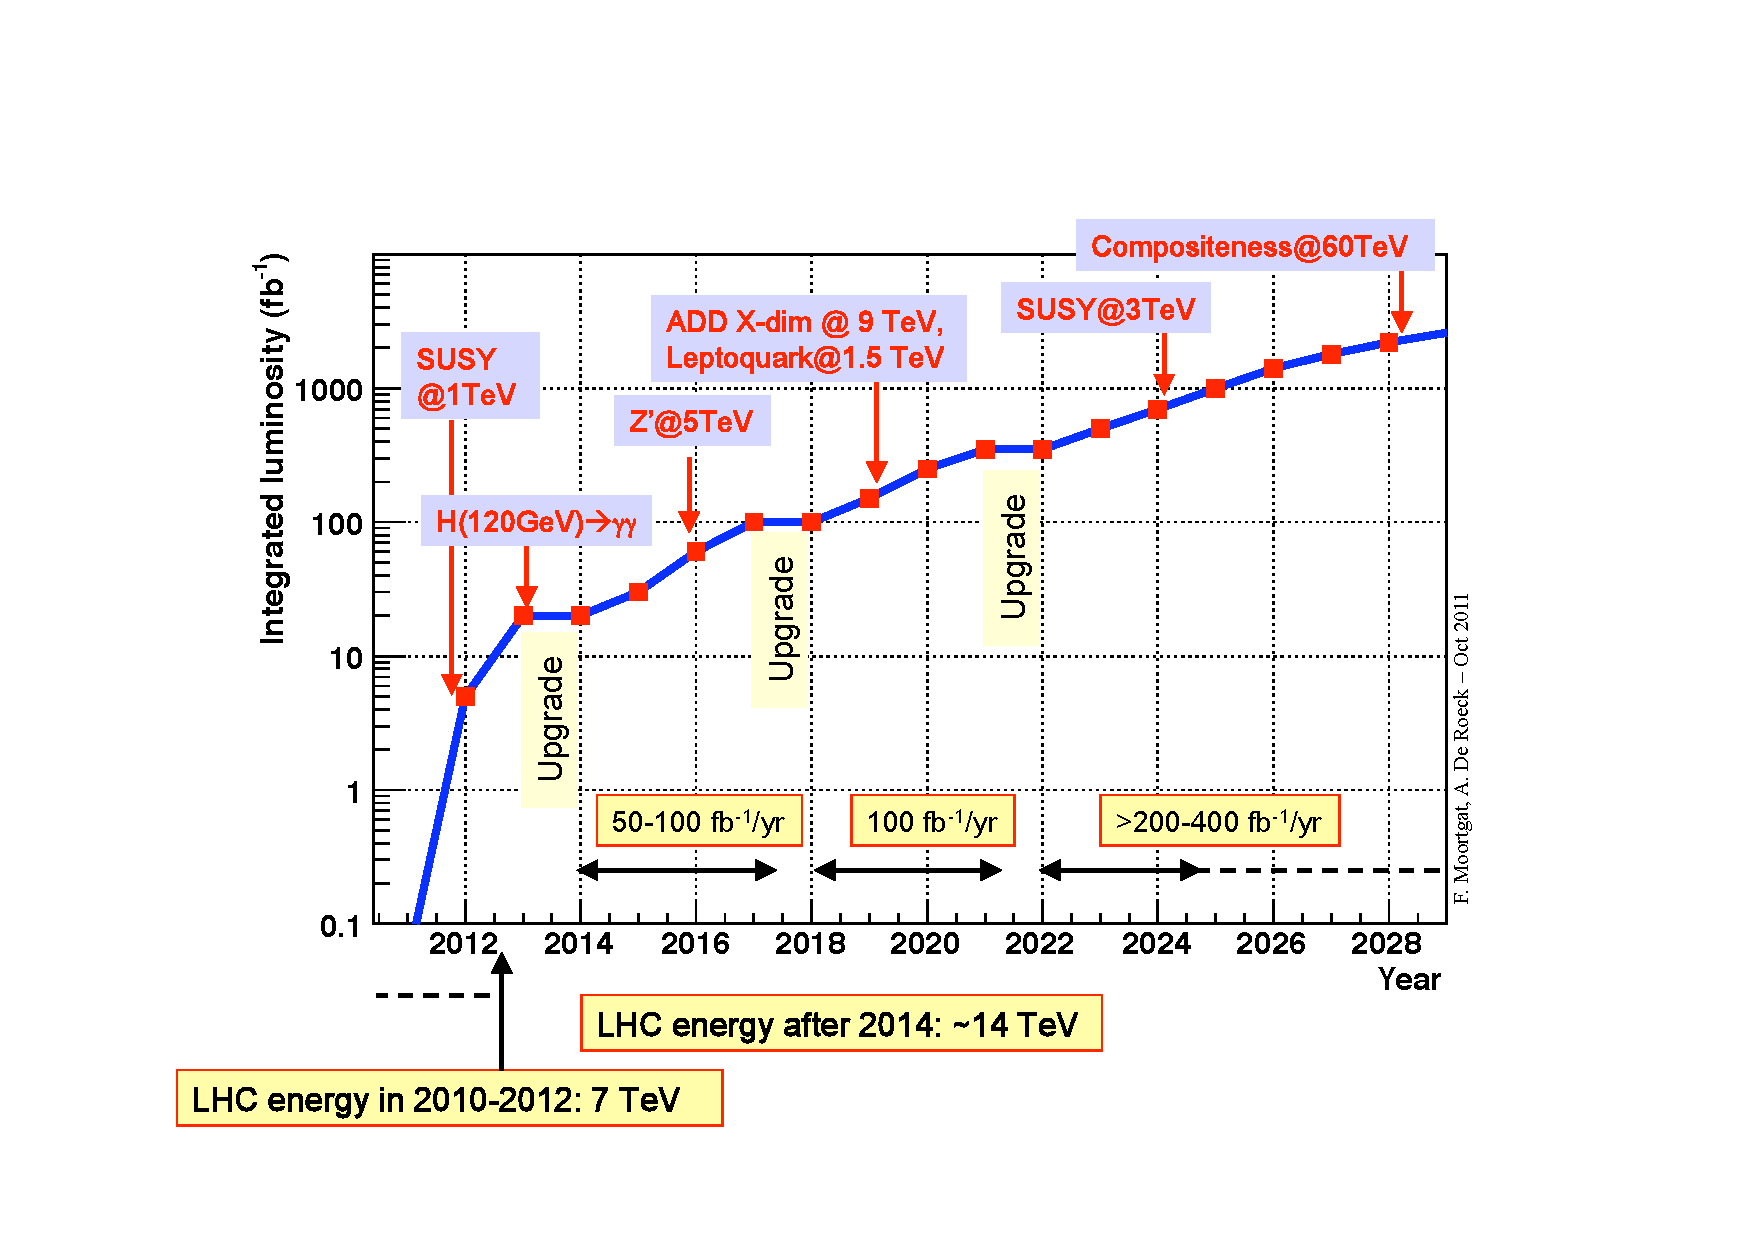
\includegraphics[width=0.45\textwidth]{Figures/pooth/schedule.pdf}
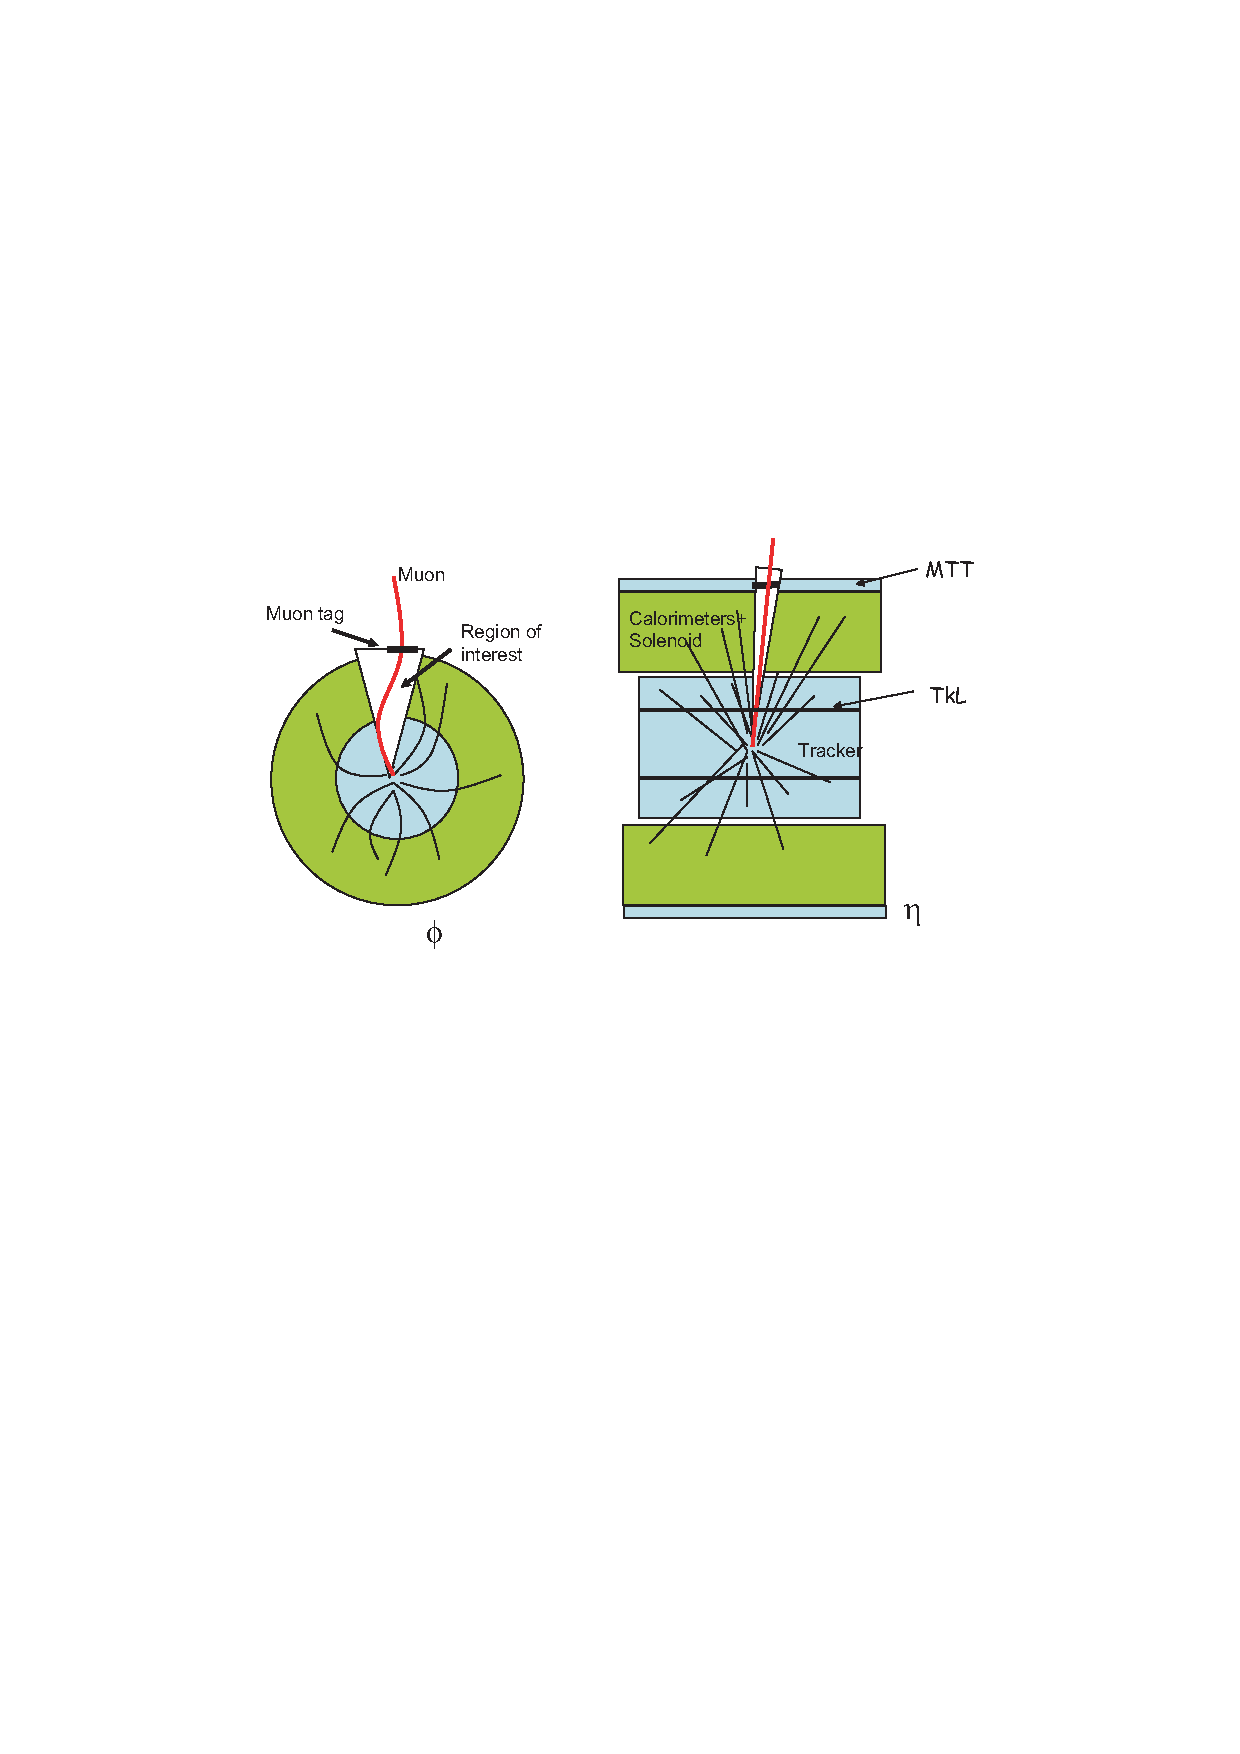
\includegraphics[width=0.52\textwidth]{Figures/pooth/mtt_concept_a.pdf}
\caption{Left: The integrated luminosity versus time for the periods before, between and after the three long shutdowns to come~\cite{schedule}. Right: The Muon Track fast Tag concept~\cite{mtt_concept}. } 
\label{fig:schedule_concept}
\end{figure}

Tiles of fast plastic scintillator material read out by silicon photomultipliers (SiPMs) are under investigation to provide the additional detector layer in the very limited space available 
between the CMS solenoid and the first muon stations. The existing outer layers of the Hadron Calorimeter (HO)  can serve as a perfect testbed for this studies. In the barrel region the 
SiPM signals of the outer layers of the Hadron Outer Calorimeter could be used in the muon trigger at Level-1. The benefits of this layer for MIP identification, punch through rejection 
and resolution of ambiguities in the DT system are described in this note. For Run II a trigger link has been established that makes the HO signals available for building Level-1 muon 
trigger primitives together with inputs from DT and RPC. Based on these data, optimization of the HO granularity for Level-1 muon triggering purposes in Phase-2 can be envisaged. 

By combining the information from various subsystems the muon momentum resolution can be improved in the Level-1 trigger system. The inner silicon based tracking system provides 
an excellent $p_t$ measurement and with the MTT it is possible to define regions of interest for the tracker in case of high $p_t$ muons. In addition the MTT can resolve possible muon 
ambiguities at very high luminosities (ghost rejection). A measured ghost and a possible solution to resolve it are shown in Figure~\ref{fig:ghosts}.
\begin{figure}[htbp]
\centering
\includegraphics[width=\textwidth]{Figures/pooth/Ghostevent01.png}
\includegraphics[width=\textwidth]{Figures/pooth/Ghostevent02.png}
\caption{Top: Four reconstructed muons (RECO mu, green crosses) with only two generated muons in the detector (GEN mu, black crosses). 
Bottom: The same event and in addition the HO system overlaid (individual HO tiles shown as pink boxes).} 
\label{fig:ghosts}
\end{figure}
\begin{figure}[htbp]
\centering
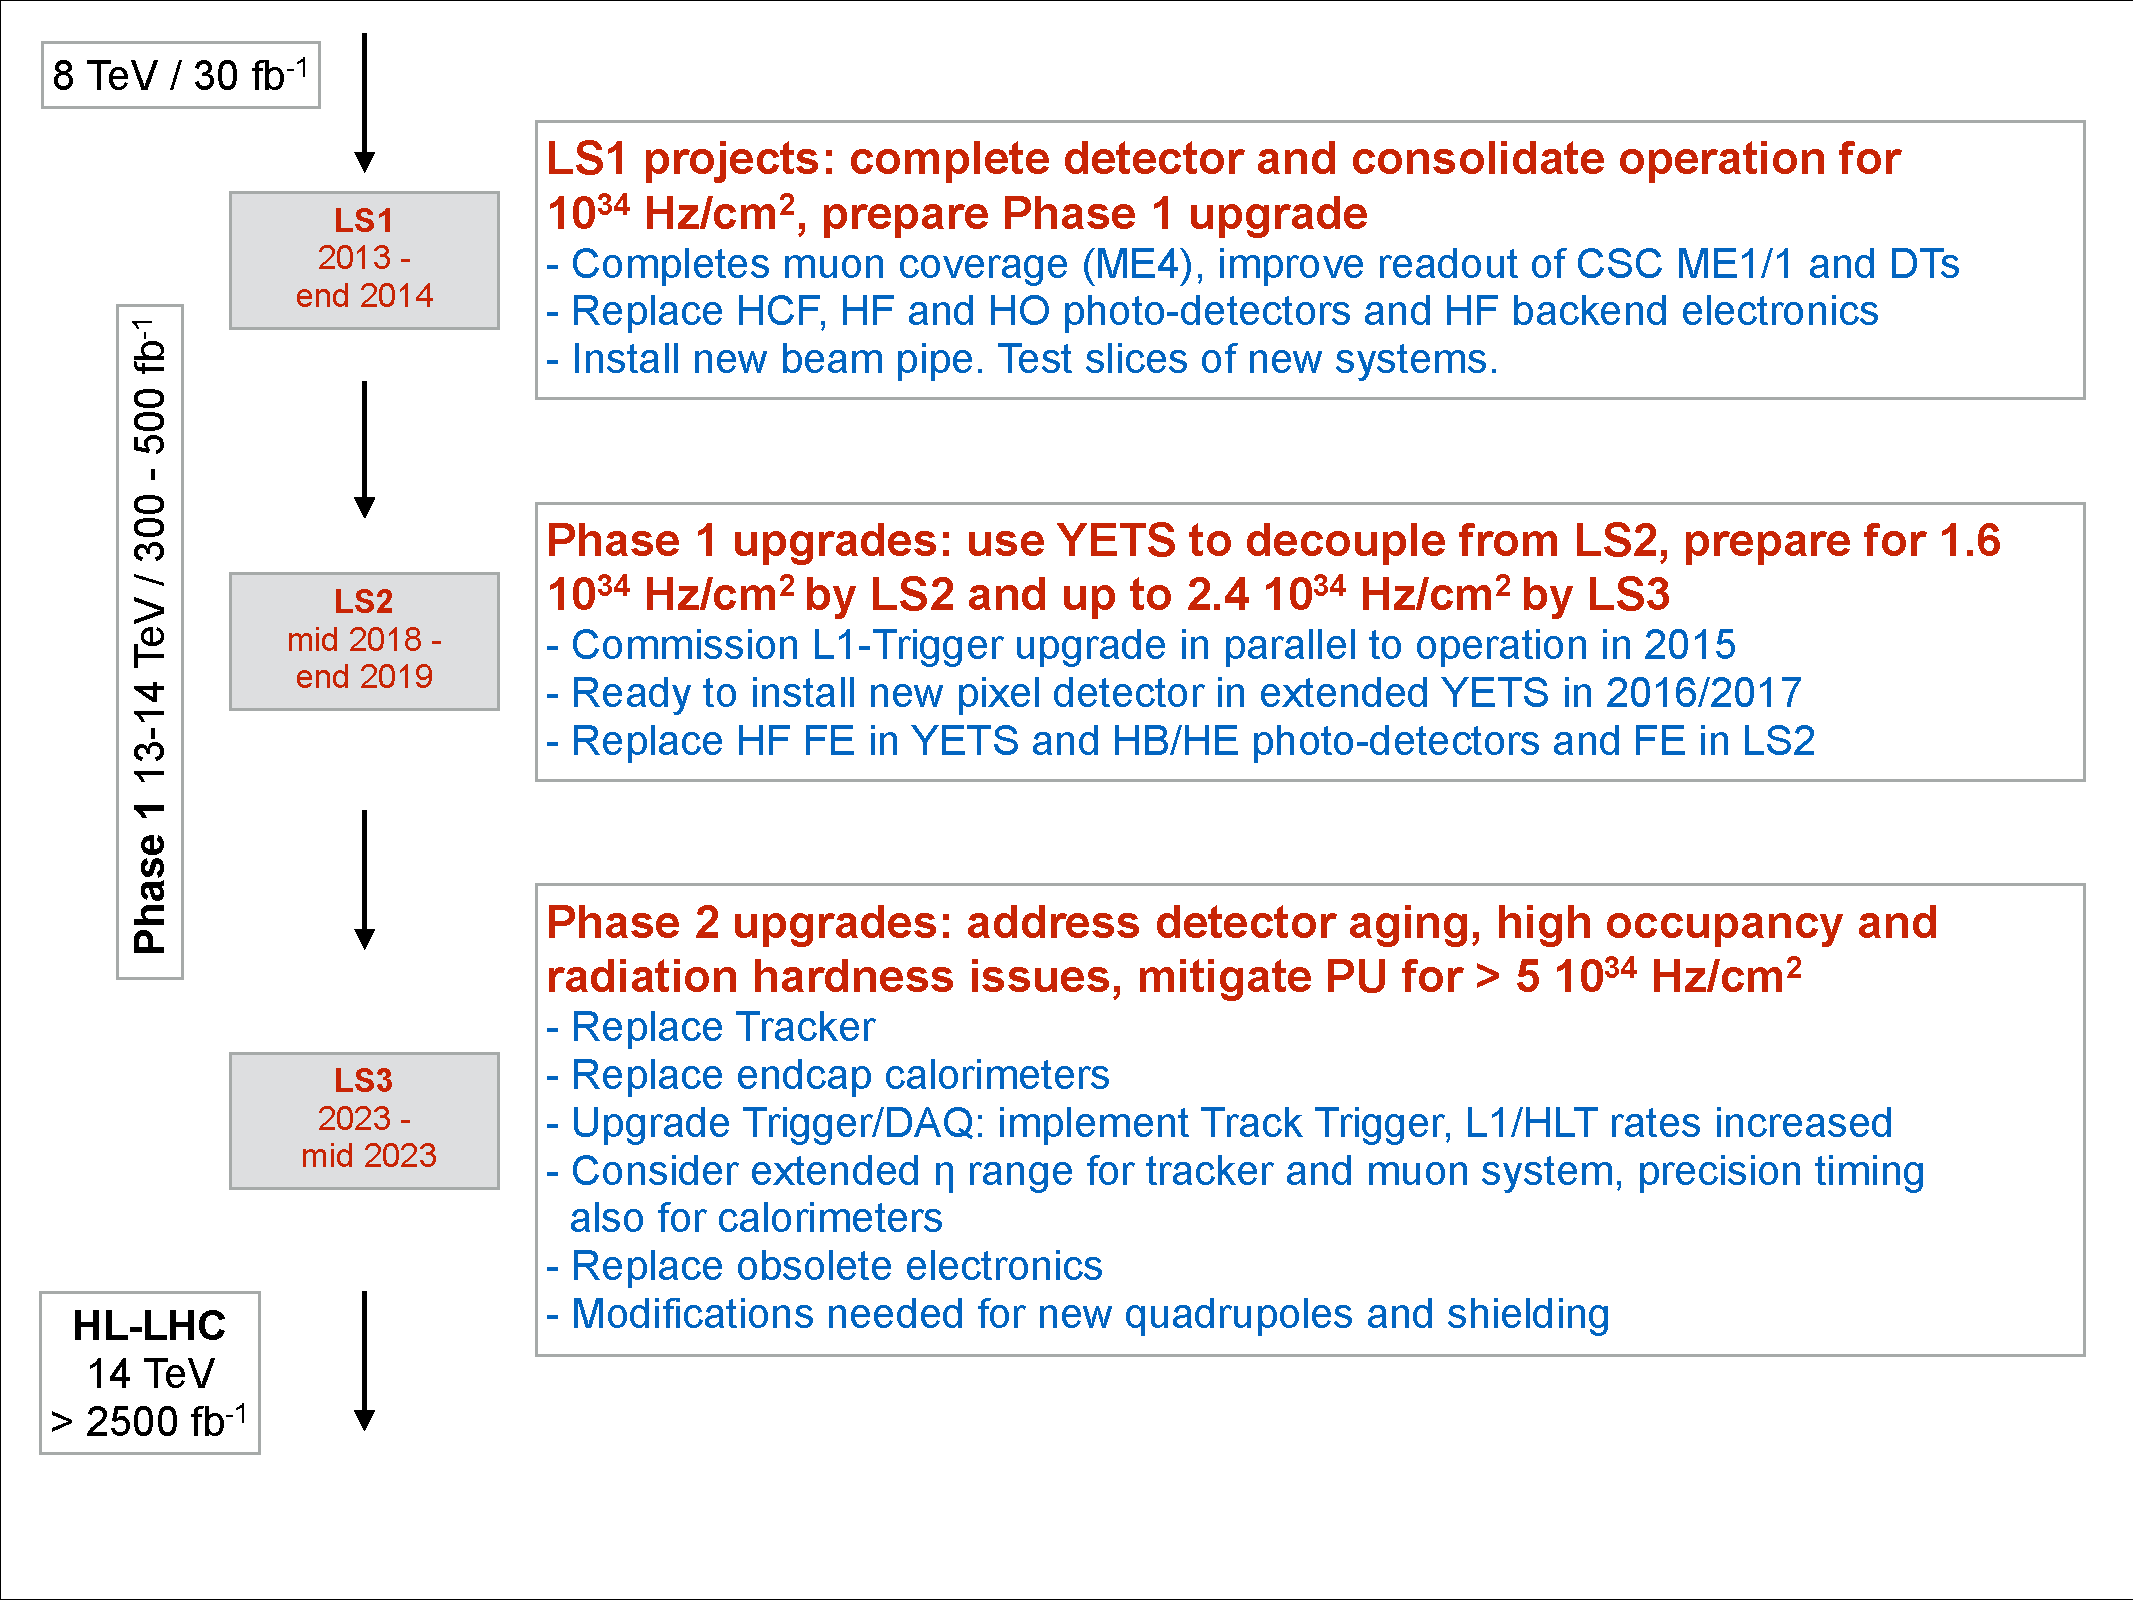
\includegraphics[width=0.8\textwidth]{Figures/pooth/upgrade_planning.pdf}\\
\caption{Upgrade planning~\cite{schedule}.} 
\label{fig:upgrade_planning}
\end{figure}
\begin{figure}[htbp]
\centering
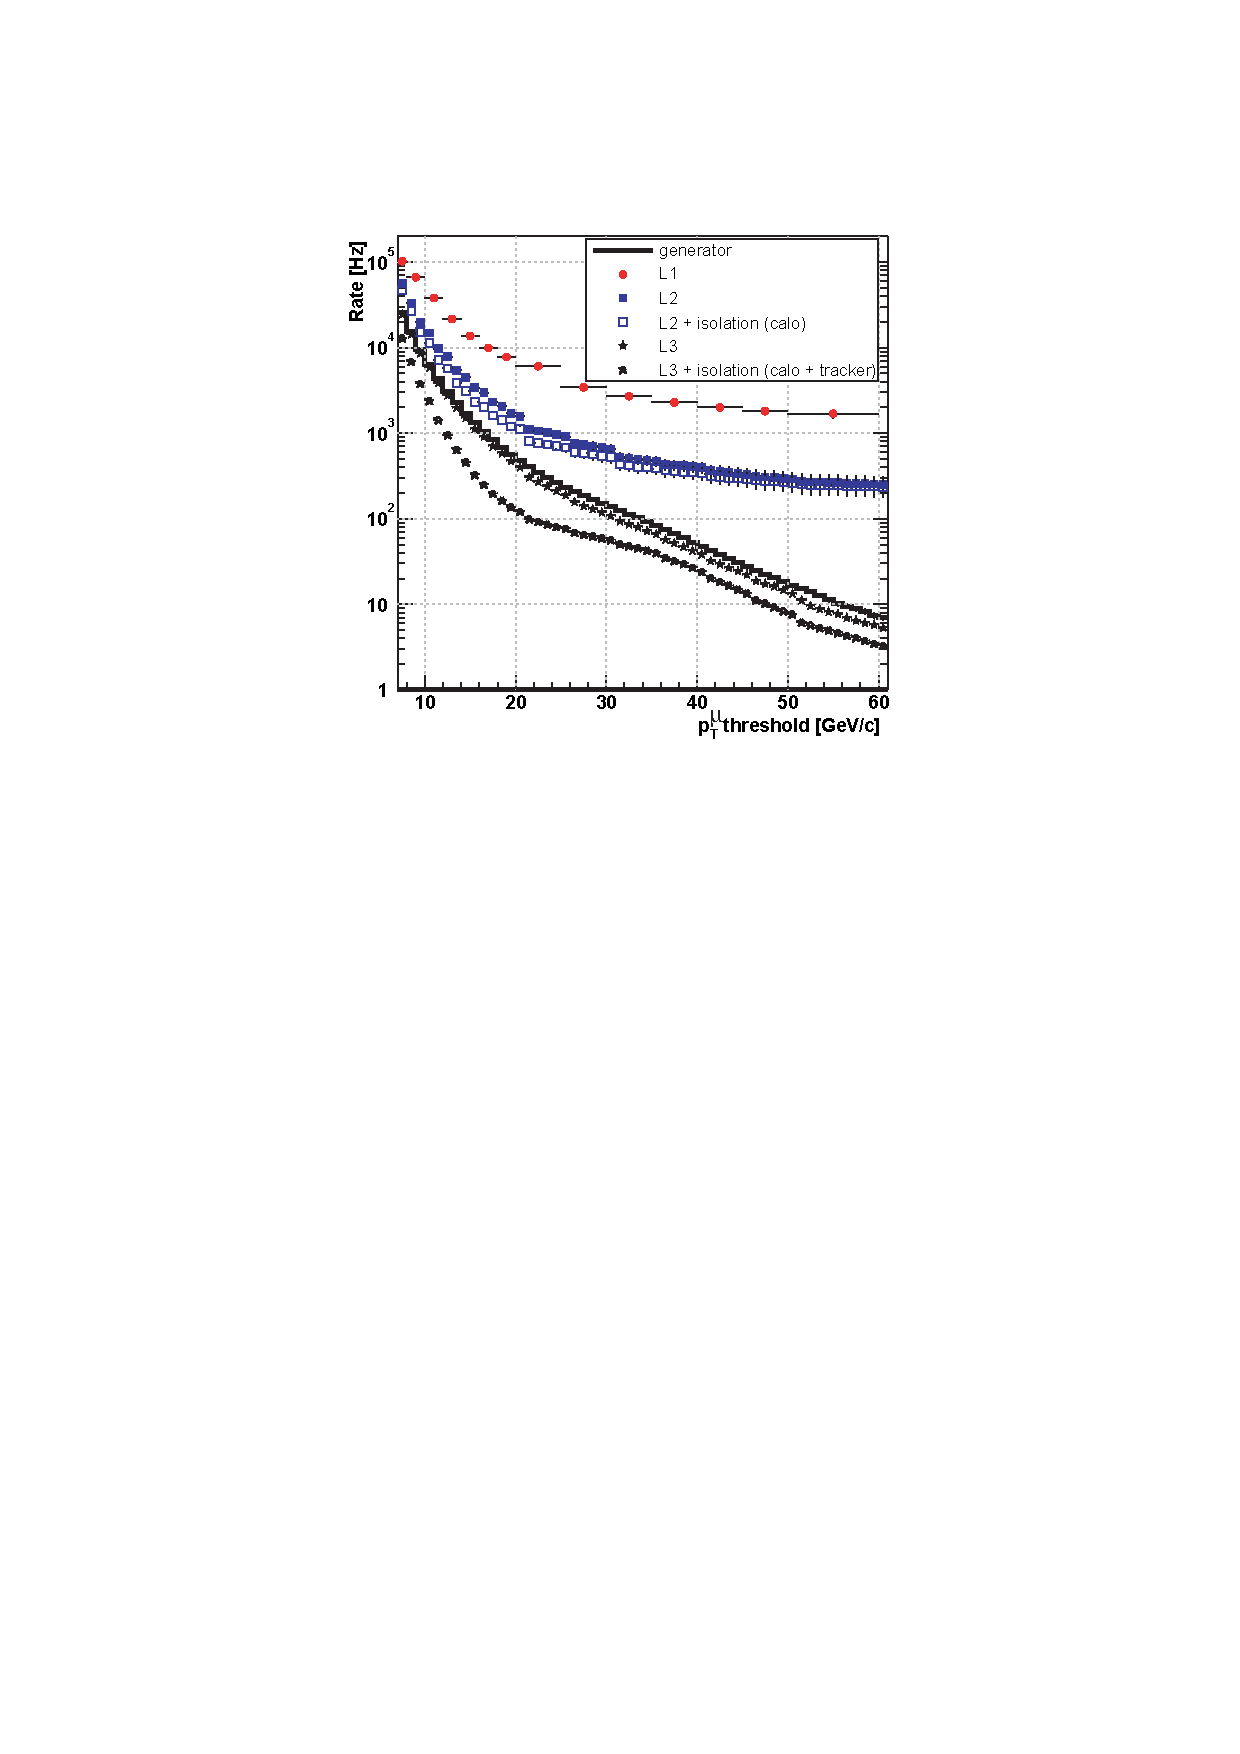
\includegraphics[width=0.5\textwidth]{Figures/pooth/pt_threshold.pdf}
\caption{Rates for different trigger levels as a function of the muon $p_t$ threshold~\cite{pt_threshold}.}
\label{fig:pt_threshold}
\end{figure}

This document is structured as follows:
\begin{itemize}
\item Prototype modules
	\begin{itemize}
	\item Silicon Photomultipliers and Frontend Electronics
	\item Measurements
	\item Simulations
	\end{itemize}
\item SiPM Upgrade in HO 
\item HO studies as an MTT testbed
\item MTT simulations in CMSSW
\item Ghost studies and interplay between MTT and existing CMS muon trigger
\end{itemize}

% >> acknowledgements (for journal papers)
% Please include the latest version from https://twiki.cern.ch/twiki/bin/viewauth/CMS/Internal/PubAcknow.
%\section*{Acknowledgements}
% ack-text

%% **DO NOT REMOVE BIBLIOGRAPHY**
\bibliography{auto_generated}   % will be created by the tdr script.

%
% Below is a multi-column format to display the standard PTDR symbols.
% Feel free to delete the lines from here to the end and the pdefs.tex file once you start modifying the template. The actual definitions are
% pulled in by the \def\Fileversion$#1: #2 ${\gdef\fileversion{#2}}
\def\Filedate$#1: #2-#3-#4 #5 ${\gdef\filedate{#2/#3/#4}}
\Fileversion$Revision: 237074 $
\Filedate$Date: 2014-04-17 15:17:42 +0200 (Thu, 17 Apr 2014) $
%%%%%%%%%%%%%%%%%%%%%%%%%%%%%%%%%%%%%%%%%%%%%%%%%%%%%%%%%%%%%%%%%%%%
%
%  CMS Common definitions style file
%
%  N.B. use of \newcommand rather than \newcommand means
%       that a definition is ignored if already specified
%
%                                              L. Taylor 18 Feb 2005
%%%%%%%%%%%%%%%%%%%%%%%%%%%%%%%%%%%%%%%%%%%%%%%%%%%%%%%%%%%%%%%%%%%%
\NeedsTeXFormat{LaTeX2e}
\ProvidesPackage{ptdr-definitions}[\filedate\space CMS Additional Physics Macros: dev version (\fileversion)]
\RequirePackage{heppennames2}
\RequirePackage{xspace}
\RequirePackage{amsmath}

% Some shorthand
% turn off italics
\newcommand {\etal}{\mbox{et al.}\xspace} %et al. - no preceding comma
\newcommand {\ie}{\mbox{i.e.}\xspace}     %i.e.
\newcommand {\eg}{\mbox{e.g.}\xspace}     %e.g.
\newcommand {\etc}{\mbox{etc.}\xspace}     %etc.
\newcommand {\vs}{\mbox{\sl vs.}\xspace}      %vs.
\newcommand {\mdash}{\ensuremath{\mathrm{-}}} % for use within formulas

% some terms whose definition we may change
\newcommand {\Lone}{Level-1\xspace} % Level-1 or L1 ?
\newcommand {\Ltwo}{Level-2\xspace}
\newcommand {\Lthree}{Level-3\xspace}

% Some software programs (alphabetized)
\newcommand{\ACERMC} {\textsc{AcerMC}\xspace}
\newcommand{\ALPGEN} {{\textsc{alpgen}}\xspace}
\newcommand{\CALCHEP} {{\textsc{CalcHEP}}\xspace}
\newcommand{\CHARYBDIS} {{\textsc{charybdis}}\xspace}
\newcommand{\CMKIN} {\textsc{cmkin}\xspace}
\newcommand{\CMSIM} {{\textsc{cmsim}}\xspace}
\newcommand{\CMSSW} {{\textsc{cmssw}}\xspace}
\newcommand{\COBRA} {{\textsc{cobra}}\xspace}
\newcommand{\COCOA} {{\textsc{cocoa}}\xspace}
\newcommand{\COMPHEP} {\textsc{CompHEP}\xspace}
\newcommand{\EVTGEN} {{\textsc{evtgen}}\xspace}
\newcommand{\FAMOS} {{\textsc{famos}}\xspace}
\newcommand{\GARCON} {\textsc{garcon}\xspace}
\newcommand{\GARFIELD} {{\textsc{garfield}}\xspace}
\newcommand{\GEANE} {{\textsc{geane}}\xspace}
\newcommand{\GEANTfour} {{\textsc{Geant4}}\xspace}
\newcommand{\GEANTthree} {{\textsc{geant3}}\xspace}
\newcommand{\GEANT} {{\textsc{geant}}\xspace}
\newcommand{\HDECAY} {\textsc{hdecay}\xspace}
\newcommand{\HERWIG} {{\textsc{herwig}}\xspace}
\newcommand{\HERWIGpp} {{\textsc{herwig++}}\xspace}
\newcommand{\POWHEG} {{\textsc{powheg}}\xspace}
\newcommand{\HIGLU} {{\textsc{higlu}}\xspace}
\newcommand{\HIJING} {{\textsc{hijing}}\xspace}
\newcommand{\IGUANA} {\textsc{iguana}\xspace}
\newcommand{\ISAJET} {{\textsc{isajet}}\xspace}
\newcommand{\ISAPYTHIA} {{\textsc{isapythia}}\xspace}
\newcommand{\ISASUGRA} {{\textsc{isasugra}}\xspace}
\newcommand{\ISASUSY} {{\textsc{isasusy}}\xspace}
\newcommand{\ISAWIG} {{\textsc{isawig}}\xspace}
\newcommand{\MADGRAPH} {\textsc{MadGraph}\xspace}
\newcommand{\MCATNLO} {\textsc{mc@nlo}\xspace}
\newcommand{\MCFM} {\textsc{mcfm}\xspace}
\newcommand{\MILLEPEDE} {{\textsc{millepede}}\xspace}
\newcommand{\ORCA} {{\textsc{orca}}\xspace}
\newcommand{\OSCAR} {{\textsc{oscar}}\xspace}
\newcommand{\PHOTOS} {\textsc{photos}\xspace}
\newcommand{\PROSPINO} {\textsc{prospino}\xspace}
\newcommand{\PYTHIA} {{\textsc{pythia}}\xspace}
\newcommand{\SHERPA} {{\textsc{sherpa}}\xspace}
\newcommand{\TAUOLA} {\textsc{tauola}\xspace}
\newcommand{\TOPREX} {\textsc{TopReX}\xspace}
\newcommand{\XDAQ} {{\textsc{xdaq}}\xspace}


%  Experiments
\newcommand {\DZERO}{D0\xspace}     %etc.


% Measurements and units...

\newcommand{\de}{\ensuremath{^\circ}}
\newcommand{\ten}[1]{\ensuremath{\times \text{10}^\text{#1}}}
\newcommand{\unit}[1]{\ensuremath{\text{\,#1}}\xspace}
\newcommand{\mum}{\ensuremath{\,\mu\text{m}}\xspace}
\newcommand{\micron}{\ensuremath{\,\mu\text{m}}\xspace}
\newcommand{\cm}{\ensuremath{\,\text{cm}}\xspace}
\newcommand{\mm}{\ensuremath{\,\text{mm}}\xspace}
\newcommand{\mus}{\ensuremath{\,\mu\text{s}}\xspace}
\newcommand{\keV}{\ensuremath{\,\text{ke\hspace{-.08em}V}}\xspace}
\newcommand{\MeV}{\ensuremath{\,\text{Me\hspace{-.08em}V}}\xspace}
\newcommand{\MeVns}{\ensuremath{\text{Me\hspace{-.08em}V}}\xspace} % no leading thinspace
\newcommand{\GeV}{\ensuremath{\,\text{Ge\hspace{-.08em}V}}\xspace}
\newcommand{\GeVns}{\ensuremath{\text{Ge\hspace{-.08em}V}}\xspace} % no leading thinspace
\newcommand{\gev}{\GeV}
\newcommand{\TeV}{\ensuremath{\,\text{Te\hspace{-.08em}V}}\xspace}
\newcommand{\TeVns}{\ensuremath{\text{Te\hspace{-.08em}V}}\xspace} % no leading thinspace
\newcommand{\PeV}{\ensuremath{\,\text{Pe\hspace{-.08em}V}}\xspace}
\newcommand{\keVc}{\ensuremath{{\,\text{ke\hspace{-.08em}V\hspace{-0.16em}/\hspace{-0.08em}}c}}\xspace}
\newcommand{\MeVc}{\ensuremath{{\,\text{Me\hspace{-.08em}V\hspace{-0.16em}/\hspace{-0.08em}}c}}\xspace}
\newcommand{\GeVc}{\ensuremath{{\,\text{Ge\hspace{-.08em}V\hspace{-0.16em}/\hspace{-0.08em}}c}}\xspace}
\newcommand{\GeVcns}{\ensuremath{{\text{Ge\hspace{-.08em}V\hspace{-0.16em}/\hspace{-0.08em}}c}}\xspace} % no leading thinspace
\newcommand{\TeVc}{\ensuremath{{\,\text{Te\hspace{-.08em}V\hspace{-0.16em}/\hspace{-0.08em}}c}}\xspace}
\newcommand{\keVcc}{\ensuremath{{\,\text{ke\hspace{-.08em}V\hspace{-0.16em}/\hspace{-0.08em}}c^\text{2}}}\xspace}
\newcommand{\MeVcc}{\ensuremath{{\,\text{Me\hspace{-.08em}V\hspace{-0.16em}/\hspace{-0.08em}}c^\text{2}}}\xspace}
\newcommand{\GeVcc}{\ensuremath{{\,\text{Ge\hspace{-.08em}V\hspace{-0.16em}/\hspace{-0.08em}}c^\text{2}}}\xspace}
\newcommand{\GeVccns}{\ensuremath{{\text{Ge\hspace{-.08em}V\hspace{-0.16em}/\hspace{-0.08em}}c^\text{2}}}\xspace} % no leading thinspace
\newcommand{\TeVcc}{\ensuremath{{\,\text{Te\hspace{-.08em}V\hspace{-0.16em}/\hspace{-0.08em}}c^\text{2}}}\xspace}

\newcommand{\pbinv} {\mbox{\ensuremath{\,\text{pb}^\text{$-$1}}}\xspace}
\newcommand{\fbinv} {\mbox{\ensuremath{\,\text{fb}^\text{$-$1}}}\xspace}
\newcommand{\nbinv} {\mbox{\ensuremath{\,\text{nb}^\text{$-$1}}}\xspace}
\newcommand{\mubinv} {\ensuremath{\,\mu\mathrm{b}^{-1}}\xspace}
\newcommand{\percms}{\ensuremath{\,\text{cm}^\text{$-$2}\,\text{s}^\text{$-$1}}\xspace}
\newcommand{\lumi}{\ensuremath{\mathcal{L}}\xspace}
\newcommand{\Lumi}{\ensuremath{\mathcal{L}}\xspace}%both upper and lower
%
% Need a convention here:
\newcommand{\LvLow}  {\ensuremath{\mathcal{L}=\text{10}^\text{32}\,\text{cm}^\text{$-$2}\,\text{s}^\text{$-$1}}\xspace}
\newcommand{\LLow}   {\ensuremath{\mathcal{L}=\text{10}^\text{33}\,\text{cm}^\text{$-$2}\,\text{s}^\text{$-$1}}\xspace}
\newcommand{\lowlumi}{\ensuremath{\mathcal{L}=\text{2}\times \text{10}^\text{33}\,\text{cm}^\text{$-$2}\,\text{s}^\text{$-$1}}\xspace}
\newcommand{\LMed}   {\ensuremath{\mathcal{L}=\text{2}\times \text{10}^\text{33}\,\text{cm}^\text{$-$2}\,\text{s}^\text{$-$1}}\xspace}
\newcommand{\LHigh}  {\ensuremath{\mathcal{L}=\text{10}^\text{34}\,\text{cm}^\text{$-$2}\,\text{s}^\text{$-$1}}\xspace}
\newcommand{\hilumi} {\ensuremath{\mathcal{L}=\text{10}^\text{34}\,\text{cm}^\text{$-$2}\,\text{s}^\text{$-$1}}\xspace}

% Physics symbols ...

\newcommand{\PT}{\ensuremath{p_{\mathrm{T}}}\xspace}
\newcommand{\pt}{\ensuremath{p_{\mathrm{T}}}\xspace}
\newcommand{\ET}{\ensuremath{E_{\mathrm{T}}}\xspace}
\newcommand{\HT}{\ensuremath{H_{\mathrm{T}}}\xspace}
\newcommand{\et}{\ensuremath{E_{\mathrm{T}}}\xspace}
\newcommand{\Em}{\ensuremath{E\hspace{-0.6em}/}\xspace}
\newcommand{\Pm}{\ensuremath{p\hspace{-0.5em}/}\xspace}
\newcommand{\PTm}{\ensuremath{{p}_\mathrm{T}\hspace{-1.02em}/\kern 0.5em}\xspace}
\newcommand{\PTslash}{\PTm}
\newcommand{\ETm}{\ensuremath{E_{\mathrm{T}}^{\text{miss}}}\xspace}
\newcommand{\MET}{\ETm}
\newcommand{\ETmiss}{\ETm}
\newcommand{\ETslash}{\ensuremath{E_{\mathrm{T}}\hspace{-1.1em}/\kern0.45em}\xspace}
\newcommand{\VEtmiss}{\ensuremath{{\vec E}_{\mathrm{T}}^{\text{miss}}}\xspace}
\newcommand{\ptvec}{\ensuremath{{\vec p}_{\mathrm{T}}}\xspace}

% roman face derivative
\newcommand{\dd}[2]{\ensuremath{\frac{\cmsSymbolFace{d} #1}{\cmsSymbolFace{d} #2}}}
\newcommand{\ddinline}[2]{\ensuremath{\cmsSymbolFace{d} #1/\cmsSymbolFace{d} #2}}
\newcommand{\rd}{\ensuremath{\cmsSymbolFace{d}}}
\newcommand{\re}{\ensuremath{\cmsSymbolFace{e}}}
% absolute value
\newcommand{\abs}[1]{\ensuremath{\lvert #1 \rvert}}



\ifthenelse{\boolean{cms@italic}}{\newcommand{\cmsSymbolFace}{\relax}}{\newcommand{\cmsSymbolFace}{\mathrm}}

% Particle names which track the italic/non-italic face convention
\newcommand{\zp}{{\PZpr}\xspace} % plain Z'
\newcommand{\JPsi}{{\PJGy}\xspace} % J/Psi (no mass)
\newcommand{\Z}{{\PZ}\xspace} % plain Z (no superscript 0)
\newcommand{\ttbar}{\PQt{}\PAQt\xspace} % t-tbar

% Extensions for missing names in PENNAMES % note no xspace, to match syntax in PENNAMES
\newcommand{\cPgn}{\PGn} % generic neutrino
\providecommand{\Pgn}{\PGn}
\newcommand{\cPagn}{\PAGn} % generic anti-neutrino
\providecommand{\Pagn}{\PAGn}
\newcommand{\cPgg}{\PGg} % gamma
\newcommand{\cPJgy}{\PJGy} % J/Psi (no mass)
\newcommand{\cPZ}{\PZ} % plain Z (no superscript 0)
\newcommand{\cPZpr}{\PZpr} % plain Z'
\newcommand{\cPqt}{\PQt} % t for t quark
\newcommand{\cPqb}{\PQb} % b for b quark
\newcommand{\cPqc}{\PQc} % c for c quark
\newcommand{\cPqs}{\PQs} % s for s quark
\newcommand{\cPqu}{\PQu} % u for u quark
\newcommand{\cPqd}{\PQd} % d for d quark
\newcommand{\cPq}{\PQq} % generic quark
\newcommand{\cPg}{\Pg} % generic gluon
\newcommand{\cPG}{\PXXG} % Graviton
\newcommand{\cPaqt}{\PAQt} % t for t anti-quark
\newcommand{\cPaqb}{\PAQb} % b for b anti-quark
\newcommand{\cPaqc}{\PAQc} % c for c anti-quark
\newcommand{\cPaqs}{\PAQs} % s for s anti-quark
\newcommand{\cPaqu}{\PAQu} % u for u anti-quark
\newcommand{\cPaqd}{\PAQd} % d for d anti-quark
\newcommand{\cPaq}{\PAQq} % generic anti-quark
\newcommand{\cPKstz}{\ensuremath{\cmsSymbolFace{K}^{\ast0}}\xspace}

% for APS style tables
\ifthenelse{\boolean{cms@external}}{%
\newenvironment{scotch}[1]{\protect\centering\ruledtabular\tabular{#1}}{\endtabular\endruledtabular}
}{
\newenvironment{scotch}[1]{\protect\centering\tabular{#1}\hline\hline}{\hline\endtabular}
}
% SM (still to be classified)

\newcommand{\AFB}{\ensuremath{A_\text{FB}}\xspace}
\newcommand{\wangle}{\ensuremath{\sin^{2}\theta_{\text{eff}}^\text{lept}(M^2_{\Z})}\xspace}
\newcommand{\stat}{\ensuremath{\,\text{(stat.)}}\xspace}
\newcommand{\syst}{\ensuremath{\,\text{(syst.)}}\xspace}
\newcommand{\lum}{\ensuremath{\,\text{(lum.)}}\xspace}
\newcommand{\kt}{\ensuremath{k_{\mathrm{T}}}\xspace}

\newcommand{\BC}{\HepParticle{B}{c}{}{}\xspace}
\newcommand{\bbarc}{\PAQb{}\PQc\xspace}
\newcommand{\bbbar}{\PQb{}\PAQb\xspace}
\newcommand{\ccbar}{\PQc{}\PAQc\xspace}
\newcommand{\bspsiphi}{\ensuremath{\PBs \to \JPsi\, \PGf}\xspace}
\newcommand{\EE}{\Pep{}\Pem\xspace}
\newcommand{\MM}{\PGmp{}\PGmm\xspace}
\newcommand{\TT}{\PGtm{}\PGtp\xspace}

%%%  E-gamma definitions
\newcommand{\HGG}{\ensuremath{\PH\to\PGg\PGg}}
\newcommand{\GAMJET}{\ensuremath{\PGg + \text{jet}}}
\newcommand{\PPTOJETS}{\ensuremath{\Pp\Pp\to\text{jets}}}
\newcommand{\PPTOGG}{\ensuremath{\Pp\Pp\to\PGg\PGg}}
\newcommand{\PPTOGAMJET}{\ensuremath{\Pp\Pp\to\PGg + \text{jet}}}
\newcommand{\MH}{\ensuremath{M_{\PH}}}
\newcommand{\RNINE}{\ensuremath{R_\mathrm{9}}}
\newcommand{\DR}{\ensuremath{\Delta R}}





%%%%%%
% From Albert
%

\newcommand{\ga}{\ensuremath{\gtrsim}}
\newcommand{\la}{\ensuremath{\lesssim}}
%
\newcommand{\swsq}{\ensuremath{\sin^2\theta_{\PW}}\xspace}
\newcommand{\cwsq}{\ensuremath{\cos^2\theta_{\PW}}\xspace}
\newcommand{\tanb}{\ensuremath{\tan\beta}\xspace}
\newcommand{\tanbsq}{\ensuremath{\tan^{2}\beta}\xspace}
\newcommand{\sidb}{\ensuremath{\sin 2\beta}\xspace}
\newcommand{\alpS}{\ensuremath{\alpha_S}\xspace}
\newcommand{\alpt}{\ensuremath{\widetilde{\alpha}}\xspace}

\newcommand{\QL}{\HepParticle{Q}{L}{}{}\xspace}
\newcommand{\sQ}{\HepSusyParticle{Q}{}{}{}\xspace}
\newcommand{\sQL}{\HepSusyParticle{Q}{L}{}{}\xspace}
\newcommand{\ULC}{\HepParticle{U}{L}{C}{}\xspace}
\newcommand{\sUC}{\HepSusyParticle{U}{}{C}{}\xspace}
\newcommand{\sULC}{\HepSusyParticle{U}{L}{C}{}\xspace}
\newcommand{\DLC}{\HepParticle{D}{L}{C}{}\xspace}
\newcommand{\sDC}{\HepSusyParticle{D}{}{C}{}\xspace}
\newcommand{\sDLC}{\HepSusyParticle{D}{L}{C}{}\xspace}
\newcommand{\LL}{\HepParticle{L}{L}{}{}\xspace}
\newcommand{\sL}{\HepSusyParticle{L}{}{}{}\xspace}
\newcommand{\sLL}{\HepSusyParticle{L}{L}{}{}\xspace}
\newcommand{\ELC}{\HepParticle{E}{L}{C}{}\xspace}
\newcommand{\sEC}{\HepSusyParticle{E}{}{C}{}\xspace}
\newcommand{\sELC}{\HepSusyParticle{E}{L}{C}{}\xspace}
\newcommand{\sEL}{\HepSusyParticle{E}{L}{}{}\xspace}
\newcommand{\sER}{\HepSusyParticle{E}{R}{}{}\xspace}
\newcommand{\sFer}{\HepSusyParticle{f}{}{}{}\xspace}
\newcommand{\sQua}{\PSQ}
\newcommand{\sUp}{\PSQu}
\newcommand{\suL}{\PSQuL}
\newcommand{\suR}{\PSQuR}
\newcommand{\sDw}{\PSQd}
\newcommand{\sdL}{\PSQdL}
\newcommand{\sdR}{\PSQdR}
\newcommand{\sTop}{\PSQt}
\newcommand{\stL}{\PSQtL}
\newcommand{\stR}{\PSQtR}
\newcommand{\stone}{\PSQtDo}
\newcommand{\sttwo}{\PSQtDt}
\newcommand{\sBot}{\PSQb}
\newcommand{\sbL}{\PSQbL}
\newcommand{\sbR}{\PSQbR}
\newcommand{\sbone}{\PSQbDo}
\newcommand{\sbtwo}{\PSQbDt}
\newcommand{\sLep}{\PSl}
\newcommand{\sLepC}{\HepSusyParticle{l}{}{C}{}\xspace}
\newcommand{\sEl}{\PSe}
\newcommand{\sElC}{\HepSusyParticle{e}{}{C}{}\xspace}
\newcommand{\seL}{\PSeL}
\newcommand{\seR}{\PSeR}
\newcommand{\snL}{\HepSusyParticle{\PGn}{L}{}{}\xspace}
\newcommand{\sMu}{\PSGm}
\newcommand{\sNu}{\PSGn}
\newcommand{\sTau}{\PSGt}
\newcommand{\Glu}{\Pg}
\newcommand{\sGlu}{\PSg}
\newcommand{\Wpm}{\PWpm}
\newcommand{\sWpm}{\PSWpm}
\newcommand{\Wz}{\HepParticle{W}{}{0}{}\xspace}
\newcommand{\sWz}{\HepSusyParticle{W}{}{0}{}\xspace}
\newcommand{\sWino}{\PSW}
\newcommand{\Bz}{\HepParticle{B}{}{0}\xspace}
\newcommand{\sBz}{\HepSusyParticle{B}{}{0}\xspace}
\newcommand{\sBino}{\HepSusyParticle{B}{}{}\xspace}
\newcommand{\Zz}{\PZz}
\newcommand{\sZino}{\PSZz}
\newcommand{\sGam}{\PSGg}
\newcommand{\chiz}{\PSGcz}
\newcommand{\chip}{\PSGcp}
\newcommand{\chim}{\PSGcm}
\newcommand{\chipm}{\PSGcpm}
\newcommand{\Hone}{\HepParticle{H}{d}{}\xspace}
\newcommand{\sHone}{\HepSusyParticle{H}{d}{}\xspace}
\newcommand{\Htwo}{\HepParticle{H}{u}{}\xspace}
\newcommand{\sHtwo}{\HepSusyParticle{H}{u}{}\xspace}
\newcommand{\sHig}{\HepSusyParticle{H}{}{}{}\xspace}
\newcommand{\sHa}{\HepSusyParticle{H}{a}{}{}\xspace}
\newcommand{\sHb}{\HepSusyParticle{H}{b}{}{}\xspace}
\newcommand{\sHpm}{\HepSusyParticle{H}{}{\pm}{}\xspace}
\newcommand{\hz}{\PShz}
\newcommand{\Hz}{\PHz}
\newcommand{\Az}{\PSAz}
\newcommand{\Hpm}{\PSHpm}
\newcommand{\sGra}{\PXXSG}
%
\newcommand{\mtil}{\ensuremath{\widetilde{m}}\xspace}
%
\newcommand{\rpv}{\ensuremath{\rlap{\kern.2em/}R}\xspace}
\newcommand{\LLE}{\ensuremath{LL\bar{E}}\xspace}
\newcommand{\LQD}{\ensuremath{LQ\bar{D}}\xspace}
\newcommand{\UDD}{\ensuremath{\overline{UDD}}\xspace}
\newcommand{\Lam}{\ensuremath{\lambda}\xspace}
\newcommand{\Lamp}{\ensuremath{\lambda'}\xspace}
\newcommand{\Lampp}{\ensuremath{\lambda''}\xspace}
%
\newcommand{\spinbd}[2]{\ensuremath{\bar{#1}_{\dot{#2}}}\xspace}

\newcommand{\MD}{\ensuremath{{M_\mathrm{D}}}\xspace}% ED mass
\newcommand{\Mpl}{\ensuremath{{M_\mathrm{Pl}}}\xspace}% Planck mass
\newcommand{\Rinv} {\ensuremath{{R}^{-1}}\xspace}

%pennames to heppenames2 translation
%no longer include mass
%PDstpm
%PKst
%
%no j subscript, no tilde
%PSHpm
%PSHz
%
%Added overbar
%PagXz
%
%Removed overbar
%PgXz
%
\newcommand{\PAz}{\PSAz}
\newcommand{\PDiz}{\PDzDoP{2420}}
\newcommand{\PDstiiz}{\PDstzDtP{2460}}
\newcommand{\PDstz}{\PDstzP{2010}}
\newcommand{\PHpm}{\PSHpm}
\newcommand{\PJgy}{\PJGyP{1S}}
\newcommand{\PKia}{\PKDoP{1400}}
\newcommand{\PKii}{\PKDtP{1770}}
\newcommand{\PKi}{\PKDoP{1270}}
\newcommand{\PKsta}{\PKstP{1370}}
\newcommand{\PKstb}{\PKstP{1680}}
\newcommand{\PKstiii}{\PKstDTP{1780}}
\newcommand{\PKstii}{\PKstDtP{1430}}
\newcommand{\PKstiv}{\PKstDfP{2045}}
\newcommand{\PKstz}{\PKstDzP{1430}}
\newcommand{\PNa}{\HepParticleResonanceFormalFull{\PN}{}{}{1440}{}{}{P}{11}{}\xspace}
\newcommand{\PNb}{\HepParticleResonanceFormalFull{\PN}{}{}{1520}{}{}{D}{13}{}\xspace}
\newcommand{\PNc}{\HepParticleResonanceFormalFull{\PN}{}{}{1535}{}{}{S}{11}{}\xspace}
\newcommand{\PNd}{\HepParticleResonanceFormalFull{\PN}{}{}{1650}{}{}{S}{11}{}\xspace}
\newcommand{\PNe}{\HepParticleResonanceFormalFull{\PN}{}{}{1675}{}{}{D}{15}{}\xspace}
\newcommand{\PNf}{\HepParticleResonanceFormalFull{\PN}{}{}{1680}{}{}{F}{15}{}\xspace}
\newcommand{\PNg}{\HepParticleResonanceFormalFull{\PN}{}{}{1700}{}{}{D}{13}{}\xspace}
\newcommand{\PNh}{\HepParticleResonanceFormalFull{\PN}{}{}{1710}{}{}{P}{11}{}\xspace}
\newcommand{\PNi}{\HepParticleResonanceFormalFull{\PN}{}{}{1720}{}{}{P}{13}{}\xspace}
\newcommand{\PNj}{\HepParticleResonanceFormalFull{\PN}{}{}{2190}{}{}{G}{17}{}\xspace}
\newcommand{\PNk}{\HepParticleResonanceFormalFull{\PN}{}{}{2220}{}{}{H}{19}{}\xspace}
\newcommand{\PNl}{\HepParticleResonanceFormalFull{\PN}{}{}{2250}{}{}{G}{19}{}\xspace}
\newcommand{\PNm}{\HepParticleResonanceFormalFull{\PN}{}{}{2600}{}{}{I}{1,11}{}\xspace}
\newcommand{\PSHz}{\HepParticle{\PSH}{}{0}{}}
\newcommand{\PSgg}{\PSGg}
\newcommand{\PSgm}{\PSGm}
\newcommand{\PSgn}{\PSGn}
\newcommand{\PSgt}{\PSGt}
\newcommand{\PSgxpm}{\PSGcpm}
\newcommand{\PSgxz}{\PSGcz}
\newcommand{\PSq}{\PSQ}
\newcommand{\PZgc}{\PZGc}
\newcommand{\PZge}{\PZGe}
\newcommand{\PZgy}{\PZGy}
\newcommand{\PZi}{\HepParticle{Z}{1}{}\xspace}
\newcommand{\PaBz}{\PABz}
\newcommand{\PaB}{\PAB}
\newcommand{\PaDz}{\PADz}
\newcommand{\PaD}{\PAD}
\newcommand{\PaKz}{\PAKz}
\newcommand{\PaSq}{\PASQ}
\newcommand{\PagL}{\PAGL}
\newcommand{\PagOp}{\HepAntiParticle{\PGO}{}{+}\xspace}
\newcommand{\PagSm}{\HepAntiParticle{\PGS}{}{-}\xspace}
\newcommand{\PagSp}{\HepAntiParticle{\PGS}{}{+}\xspace}
\newcommand{\PagSz}{\HepAntiParticle{\PGS}{}{0}\xspace}
\newcommand{\PagXp}{\HepAntiParticle{\PGX}{}{+}\xspace}
\newcommand{\PagXz}{\HepAntiParticle{\PGX}{}{0}\xspace}
\newcommand{\Pagne}{\PAGne}
\newcommand{\Pagngm}{\PAGnGm}
\newcommand{\Pagngt}{\PAGnGt}
\newcommand{\Paii}{\PaDtP{1320}}
\newcommand{\Pai}{\PaDoP{1260}}
\newcommand{\Pap}{\PAp}
\newcommand{\Paqb}{\PAQqb}
\newcommand{\Paqc}{\PAQqc}
\newcommand{\Paqd}{\PAQqd}
\newcommand{\Paqs}{\PAQqs}
\newcommand{\Paqt}{\PAQqt}
\newcommand{\Paqu}{\PAQqu}
\newcommand{\Paq}{\PAQq}
\newcommand{\Paz}{\PaDzP{980}}
\newcommand{\Pbgcia}{\PGcbDoP{2P}}
\newcommand{\Pbgciia}{\PGcbDtP{2P}}
\newcommand{\Pbgcii}{\PGcbDtP{1P}}
\newcommand{\Pbgci}{\PGcbDoP{1P}}
\newcommand{\Pbgcza}{\PGcbDzP{2P}}
\newcommand{\Pbgcz}{\PGcbDzP{1P}}
\newcommand{\Pbi}{\PbDoP{1235}}
\newcommand{\PcgLp}{\PGLpc}
\newcommand{\PcgS}{\PGScP{2455}}
\newcommand{\PcgXp}{\PGXpc}
\newcommand{\PcgXz}{\PGXzc}
\newcommand{\Pcgcii}{\PGccDtP{1P}}
\newcommand{\Pcgci}{\PGccDoP{1P}}
\newcommand{\Pcgcz}{\PGccDzP{1S}}
\newcommand{\Pcgh}{\PGhcP{1S}}
\newcommand{\Pfia}{\PfDoP{1390}}
\newcommand{\Pfib}{\PfDoP{1510}}
\newcommand{\Pfiia}{\PfDtP{1720}}
\newcommand{\Pfiib}{\PfDtP{2010}}
\newcommand{\Pfiic}{\PfDtP{2300}}
\newcommand{\Pfiid}{\PfDtP{2340}}
\newcommand{\Pfiipr}{\PfprDtP{1525}}
\newcommand{\Pfii}{\PfDtP{1270}}
\newcommand{\Pfiv}{\PfDfP{2050}}
\newcommand{\Pfi}{\PfDoP{1285}}
\newcommand{\Pfza}{\PfDzP{1400}}
\newcommand{\Pfzb}{\PfDzP{1590}}
\newcommand{\Pfz}{\PfDzP{975}}
\newcommand{\PgD}{\PGD}
\newcommand{\PgDa}{\HepParticleResonanceFormalFull{\PGD}{}{}{1232}{}{}{P}{33}{}\xspace}
\newcommand{\PgDb}{\HepParticleResonanceFormalFull{\PGD}{}{}{1620}{}{}{S}{31}{}\xspace}
\newcommand{\PgDc}{\HepParticleResonanceFormalFull{\PGD}{}{}{1700}{}{}{D}{33}{}\xspace}
\newcommand{\PgDd}{\HepParticleResonanceFormalFull{\PGD}{}{}{1900}{}{}{S}{31}{}\xspace}
\newcommand{\PgDe}{\HepParticleResonanceFormalFull{\PGD}{}{}{1905}{}{}{F}{35}{}\xspace}
\newcommand{\PgDf}{\HepParticleResonanceFormalFull{\PGD}{}{}{1910}{}{}{P}{31}{}\xspace}
\newcommand{\PgDh}{\HepParticleResonanceFormalFull{\PGD}{}{}{1920}{}{}{P}{33}{}\xspace}
\newcommand{\PgDi}{\HepParticleResonanceFormalFull{\PGD}{}{}{1930}{}{}{D}{35}{}\xspace}
\newcommand{\PgDj}{\HepParticleResonanceFormalFull{\PGD}{}{}{1950}{}{}{F}{37}{}\xspace}
\newcommand{\PgDk}{\HepParticleResonanceFormalFull{\PGD}{}{}{2420}{}{}{H}{3,11}{}\xspace}
\newcommand{\PgL}{\PGL}
\newcommand{\PgLa}{\HepParticleResonanceFormalFull{\PGL}{}{}{1405}{}{}{S}{01}{}}
\newcommand{\PgLb}{\HepParticleResonanceFormalFull{\PGL}{}{}{1520}{}{}{D}{03}{}}
\newcommand{\PgLc}{\HepParticleResonanceFormalFull{\PGL}{}{}{1600}{}{}{P}{01}{}}
\newcommand{\PgLd}{\HepParticleResonanceFormalFull{\PGL}{}{}{1670}{}{}{S}{01}{}}
\newcommand{\PgLe}{\HepParticleResonanceFormalFull{\PGL}{}{}{1690}{}{}{D}{03}{}}
\newcommand{\PgLf}{\HepParticleResonanceFormalFull{\PGL}{}{}{1800}{}{}{S}{01}{}}
\newcommand{\PgLg}{\HepParticleResonanceFormalFull{\PGL}{}{}{1810}{}{}{P}{01}{}}
\newcommand{\PgLh}{\HepParticleResonanceFormalFull{\PGL}{}{}{1820}{}{}{F}{05}{}}
\newcommand{\PgLi}{\HepParticleResonanceFormalFull{\PGL}{}{}{1830}{}{}{D}{05}{}}
\newcommand{\PgLj}{\HepParticleResonanceFormalFull{\PGL}{}{}{1890}{}{}{P}{03}{}}
\newcommand{\PgLk}{\HepParticleResonanceFormalFull{\PGL}{}{}{2100}{}{}{G}{07}{}}
\newcommand{\PgLl}{\HepParticleResonanceFormalFull{\PGL}{}{}{2110}{}{}{F}{05}{}}
\newcommand{\PgLm}{\HepParticleResonanceFormalFull{\PGL}{}{}{2350}{}{}{H}{09}{}}
\newcommand{\PgO}{\PGO}
\newcommand{\PgOm}{\PGOm}
\newcommand{\PgOma}{\PGOmP{2250}}
\newcommand{\PgS}{\PGS}
\newcommand{\PgSa}{\HepParticleResonanceFormalFull{\PGS}{}{}{1385}{}{}{P}{13}{}\xspace}
\newcommand{\PgSb}{\HepParticleResonanceFormalFull{\PGS}{}{}{1660}{}{}{P}{11}{}\xspace}
\newcommand{\PgSc}{\HepParticleResonanceFormalFull{\PGS}{}{}{1670}{}{}{D}{13}{}\xspace}
\newcommand{\PgSd}{\HepParticleResonanceFormalFull{\PGS}{}{}{1750}{}{}{S}{11}{}\xspace}
\newcommand{\PgSe}{\HepParticleResonanceFormalFull{\PGS}{}{}{1775}{}{}{D}{15}{}\xspace}
\newcommand{\PgSf}{\HepParticleResonanceFormalFull{\PGS}{}{}{1915}{}{}{F}{15}{}\xspace}
\newcommand{\PgSg}{\HepParticleResonanceFormalFull{\PGS}{}{}{1940}{}{}{D}{13}{}\xspace}
\newcommand{\PgSh}{\HepParticleResonanceFormalFull{\PGS}{}{}{2030}{}{}{F}{17}{}\xspace}
\newcommand{\PgSi}{\PGSP{2050}}
\newcommand{\PgSm}{\PGSm}
\newcommand{\PgSp}{\PGSp}
\newcommand{\PgSz}{\PGSz}
\newcommand{\PgU}{\PGU}
\newcommand{\PgUa}{\PGUP{1S}}
\newcommand{\PgUb}{\PGUP{2S}}
\newcommand{\PgUc}{\PGUP{3S}}
\newcommand{\PgUd}{\PGUP{4S}}
\newcommand{\PgUe}{\PGUP{10860}}
\newcommand{\PgUf}{\PGUP{11020}}
\newcommand{\PgX}{\PGX}
\newcommand{\PgXa}{\HepParticleResonanceFormalFull{\PGX}{}{}{1530}{}{}{P}{13}{}\xspace}
\newcommand{\PgXb}{\PGXP{1690}}
\newcommand{\PgXc}{\HepParticleResonanceFormalFull{\PGX}{}{}{1820}{}{}{D}{13}{}\xspace}
\newcommand{\PgXd}{\PGXP{1950}}
\newcommand{\PgXe}{\PGXP{2030}}
\newcommand{\PgXm}{\PGXm}
\newcommand{\PgXz}{\HepParticle{\PGX}{}{0}{}}
\newcommand{\Pgfa}{\PGfP{1680}}
\newcommand{\Pgfiii}{\PGfDTP{1850}}
\newcommand{\Pgf}{\PGfP{1020}}
\newcommand{\Pgg}{\PGg}
\newcommand{\Pgha}{\PGhP{1295}}
\newcommand{\Pghb}{\PGhP{1440}}
\newcommand{\Pghpr}{\PGhprP{958}}
\newcommand{\Pgh}{\PGh}
\newcommand{\Pgmm}{\PGmm}
\newcommand{\Pgmp}{\PGmp}
\newcommand{\Pgm}{\PGm}
\newcommand{\Pgne}{\PGne}
\newcommand{\Pgngm}{\PGnGm}
\newcommand{\Pgngt}{\PGnGt}
\newcommand{\Pgoa}{\PGoP{1390}}
\newcommand{\Pgob}{\PGoP{1600}}
\newcommand{\Pgoiii}{\PGoDTP{1670}}
\newcommand{\Pgo}{\PGoP{783}}
\newcommand{\Pgpa}{\PGpP{1300}}
\newcommand{\Pgpii}{\PGpDtP{1670}}
\newcommand{\Pgpm}{\PGpm}
\newcommand{\Pgppm}{\PGppm}
\newcommand{\Pgpp}{\PGpp}
\newcommand{\Pgpz}{\PGpz}
\newcommand{\Pgp}{\PGp}
\newcommand{\Pgra}{\PGrP{1450}}
\newcommand{\Pgrb}{\PGrP{1700}}
\newcommand{\Pgriii}{\PGrDTP{1690}}
\newcommand{\Pgr}{\PGrP{770}}
\newcommand{\Pgt}{\PGt}
\newcommand{\Pgya}{\PGyP{3770}}
\newcommand{\Pgyb}{\PGyP{4040}}
\newcommand{\Pgyc}{\PGyP{4160}}
\newcommand{\Pgyd}{\PGyP{4415}}
\newcommand{\Pgy}{\PGyP{2S}}
\newcommand{\Phia}{\PhDoP{1170}}
\newcommand{\Pqb}{\PQqb}
\newcommand{\Pqc}{\PQqc}
\newcommand{\Pqd}{\PQqd}
\newcommand{\Pqs}{\PQqs}
\newcommand{\Pqt}{\PQqt}
\newcommand{\Pqu}{\PQqu}
\newcommand{\Pq}{\PQq}
\newcommand{\PsDipm}{\PDpmsDoP{2536}}
\newcommand{\PsDm}{\PDms}
\newcommand{\PsDp}{\PDps}
\newcommand{\PsDst}{\HepParticle{\PD}{s}{\ast}\xspace}
%
\endinput
 at the beginning.
%
